\documentclass[12pt,a4paper]{scrartcl}
\usepackage[english]{babel}
\usepackage{url}
\usepackage{hyperref}

\hypersetup{
	colorlinks=true,
	urlcolor=black,
	linkcolor=black,
	citecolor=black
}
\usepackage{float}
\usepackage{graphicx}
\usepackage{listings}
\usepackage{amsmath}

\title{\large{Highly Available, Distributed and Fault Tolerant Storage System} \\ \normalsize{Distributed Systems 2011}}
\author{Karsten Westra\\1693905 \and Edwin-Jan Harmsma\\1735535}

\begin{document}
\maketitle

\tableofcontents
\clearpage


% @karsten: ik heb 'problem statement' en 'state of the art' omgewisseld
% omdat ik state of the art meer bij solution vind horen...

\section{Context}
% basics principles of storage systems
% key->value, distributed file systems, memcache
% introduce fault-tolerance (replication) and scalability

\section{Problem statement}
% introduce all requirements of our system
% show get, add, delete, set operations
% communication between different platforms
% show that basic idea is the same as file system (free list, file table, raw storage).

\section{State of the Art}
\label{sec:state-of-the-art}
% introduce XOR idea (raid4 and raid5)


\begin{figure}[H]
\centering
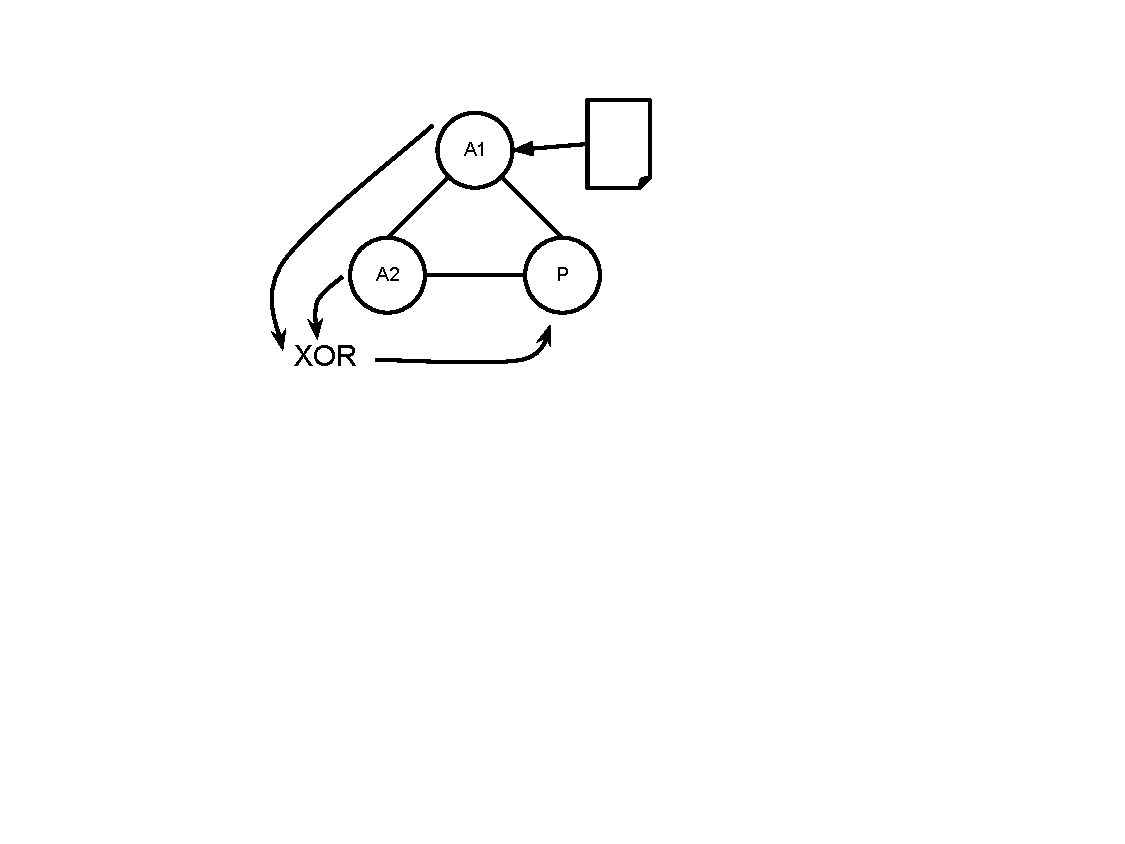
\includegraphics[width=0.5\textwidth,trim=4cm 8cm 8cm 1cm,clip=true]{diagrams/xor-replication.pdf}
\caption{XOR replication principle (RAID4)}
\label{fig:xor-replication}
\end{figure}

% asynchronous client-server, FIFO channels
% removing consistency issues --> less communication between instances 
% binary header-based protocol (platform independent)
% no block size for storage
% hash signing for security, client collects data by itself
% keeping connections open --> import for connection between storage services

\section{Solution details}
The layered architecture of the entire system is shown in \autoref{fig:layers}. There exist three layers, where the front-end layer below the client is optional. This layer is intended to make the client layer less complex and to improve some potential security issues, since it will hide all information about the actual underlying server infrastructure. With a front-end layer the client cannot trace the actual server instance that is storing a specific piece of a file or the actual server instance that stores the key of the file. Normally, this is not a very important issue, but it could make for example distributed denial-of-service attacks more easy.

The two arrows in \autoref{fig:layers} display the two different interfaces that are seen by the client. As mentioned above, if the front-end layer will be used the client will only use the use the public interface (GET, ADD, DELETE) that is indicated by \emph{arrow 1}. The front-end layer will forward this to the right dictionary server and collect the data from the storage service instances. \emph{Arrow 2} indicates the low level storage interface (READ, WRITE) that the client will use to respectively read or write the content of an entity. This interface might at first sight look a security vulnerability, but remember that the client can only use this interface with a valid timestamped signature that is granted by the dictionary service (by \emph{arrow 1}). So, this must ensure that it is impossible to write or read data randomly from a storage server, and this also explains why the front-end layer is optional.

\begin{figure}[H]
\centering
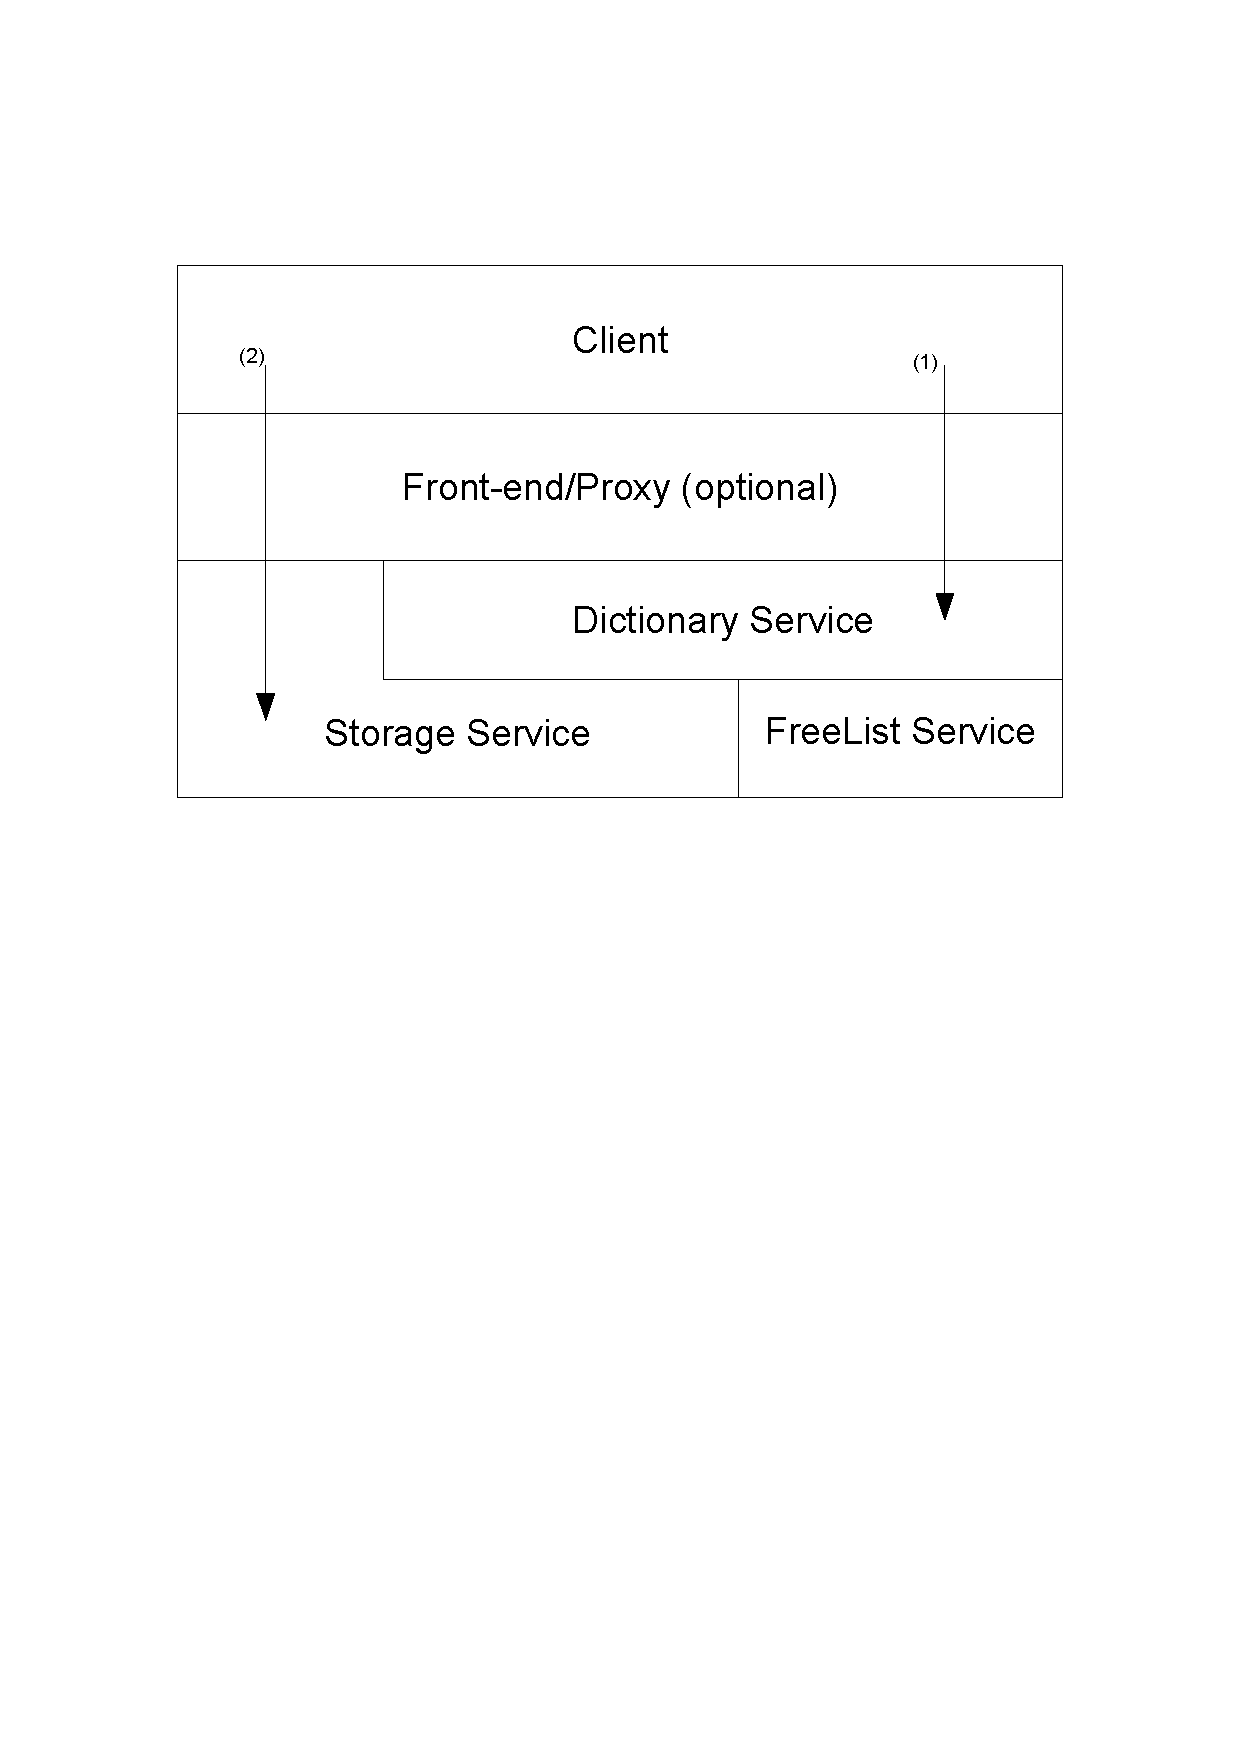
\includegraphics[width=0.8\textwidth,trim=1cm 16cm 1cm 4cm,clip=true]{diagrams/layer-architecture.pdf}
\caption{Layered architecture}
\label{fig:layers}
\end{figure}

In \autoref{fig:sequence-add} the sequence diagram of the ADD operation is shown. The ADD operation is shown because it is the most complex operation of all because it involves all other components. The front-end layer is not present in this diagram and the client will thus directly communicate with the Dictionary Services and Storage Services. Note that all objects in this diagram are distributed and require communication over a network. Also, the diagram suggests that for example \verb|write(offset, data)| completes in one step, but this is not the case in real life. Usually, these write actions are performed in multiple steps caused by of the buffering behavior of the underlying network  and the use of a network event library.

\begin{figure}[H]
\centering
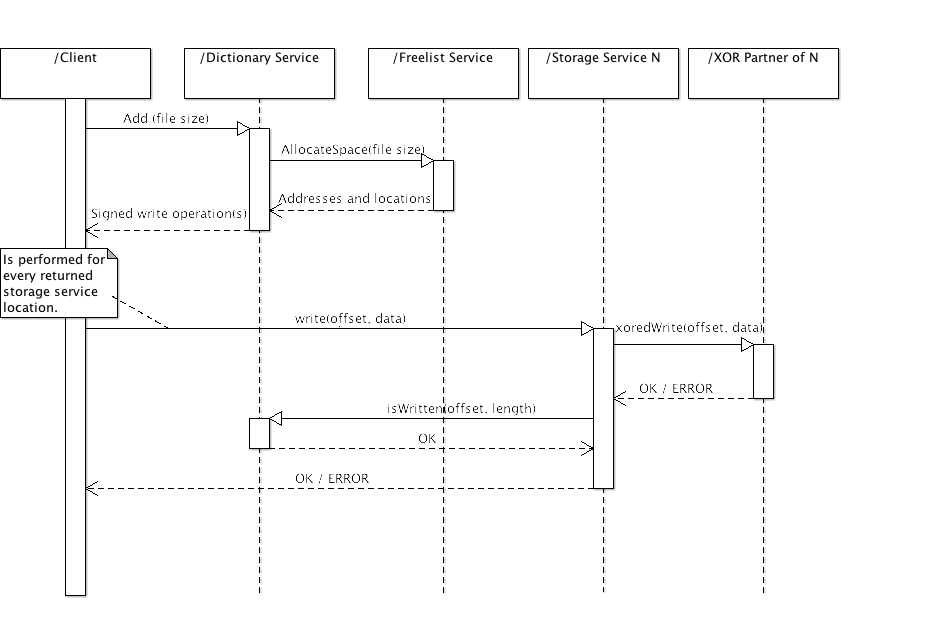
\includegraphics[width=\textwidth,trim=0 2cm 3cm 1cm,clip=true]{diagrams/add-operation.png}
\caption{Sequence diagram of the ADD operation. (Distributed communication within Dictionary Service and Freelist Service is not displayed for simplicity reasons.)}
\label{fig:sequence-add}
\end{figure}

The following subsections will discuss all the individual layers in more detail.


\subsection{Storage Service}
The storage Service is with the Freelist Service the lowest layer in the architecture and only contains a very low level API that only allows \verb|READ|, \verb|WRITE| and \verb|XORED_WRITE| operations.

\paragraph{Communication interface}
The public (and internal) storage interface is relatively simple and is defined by the following three Protocol Buffer messages:
\begin{verbatim}
message HashedStorageHeader {
    enum HashAlgorithm {
        SHA1 = 1;
    }
    required HashAlgorithm hashAlgorithm = 1;
    required bytes hash = 2;
    required StorageHeader header = 3;
}

message StorageHeader {
    enum Operation {
        READ = 1;
        WRITE = 2;
        XOR_WRITE = 3;
    }
    required Operation operation = 1;
    required uint64 offset = 2;
    required uint64 length = 3;
    required uint64 requestTimestamp = 4;
}

message StorageResponseHeader {
    enum Status {
        OK = 1;
        ERROR = 2;
    }
    required Status status = 1;
    required StorageHeader header = 2;
    optional string errorMsg = 3; // is set if status == ERROR
}
\end{verbatim}
Clients can send \verb|HashedStorageHeader| optionally followed by \emph{length} number of raw bytes in case of \verb|XORED_WRITE| and \verb|WRITE| operations to a storage service instance. The storage service sends a \verb|StorageResponseHeader| message back to the client.

\paragraph{Security}
The \verb|HashedStorageHeader| contain a signature that gives access to the file for a certain amount of time (30 seconds in the current implementation). This means that a client is allowed to \emph{write to} or \emph{read from} the given offset and length for this amount of time, after the sign has expired the client must send a new request to the dictionary service. The signature is created by talking the \emph{SHA1} hashsum of the entire nested \verb|StorageHeader| message (including timestamp) concatenated with a private key that is known by the dictionary service and storage service. Note that this private key must be unique for every storage service because the server address is not part of the signature.

The above principle ensures that only the dictionary service can grant access to clients, and that they can only perform the requested operation within a certain amount of time. However, with this principle there is still a dangerous security problem. Now, an evil client could request the dictionary service for an ADD operation and immediately after it a GET operation without actually executing the write. In this case, the client can now perform the GET operation and read the old data that possibly contains privacy sensitive information.
For this reason, we have decided that the storage service must always notify the dictionary service if a piece of file is actually written (i.e. the \emph{length} bytes are actually received from the client after a \verb|WRITE| request). The dictionary service will never grant access for a \verb|READ| before this notification is received from the storage service, thus \verb|READ| operations are never allowed before the \verb|WRITE| operation is finished.

The timestamped hashing principle ensures that clients cannot read or write data that is not intended for them. However, it is also required that eavesdropping and man-in-the-middle attacks are prevented, this is ensured by using the SSL encryption layer.

\paragraph{Asynchronous event based communication}
Since we use the Python Twisted asynchronous event framework, the implementation of the protocol parser is also created in this project. The problem of non-blocking IO is that you don't know how much data is received per event, and you don't know in advance if this is enough to parse the entire message. It was for this reason necessary to prepend the length of the message in front of the actual message data as shown in \autoref{fig:message-structure}. %TODO add reference: http://code.google.com/intl/nl-NL/apis/protocolbuffers/docs/techniques.html#streaming
In this way, we are able to stream multiple messages over the same connection, this is very useful for the replication connection that is explained in the following section.

\begin{figure}[H]
\centering
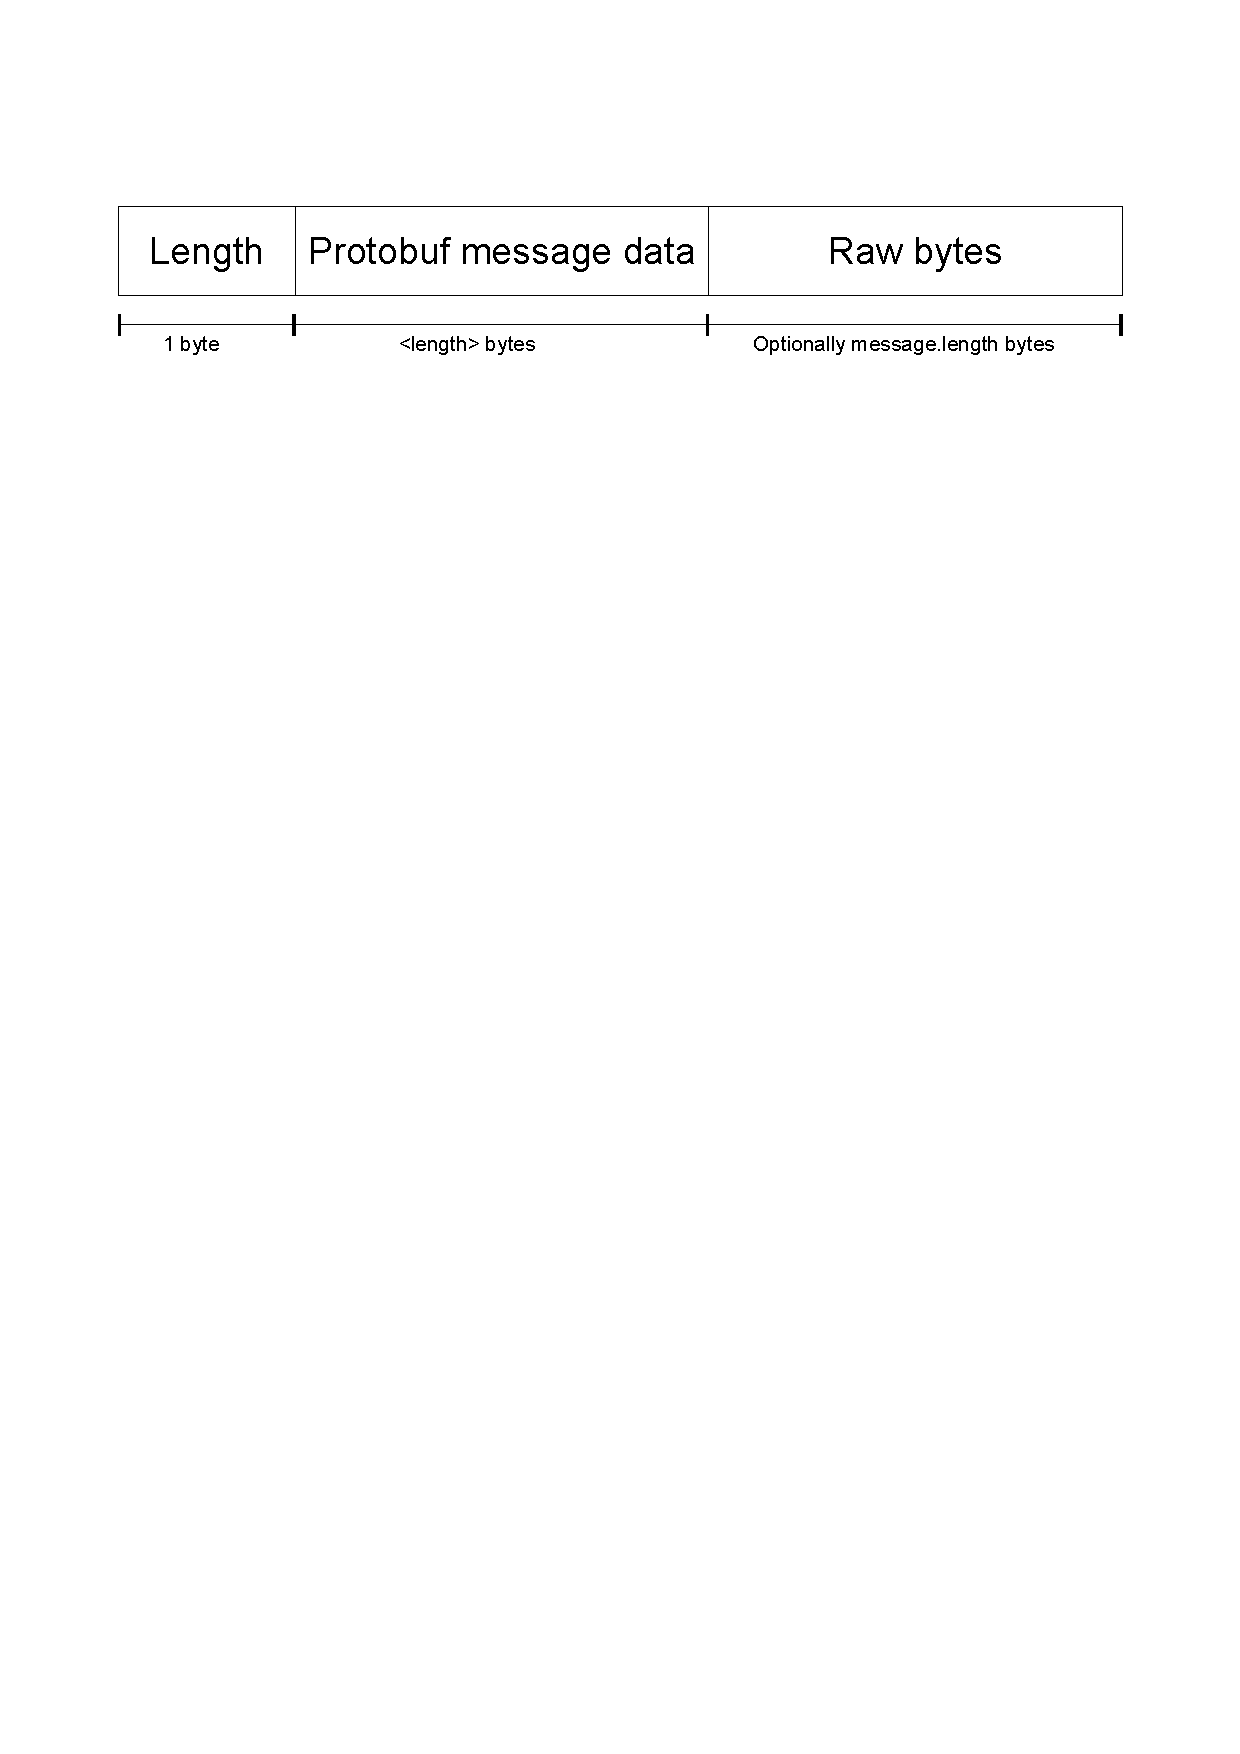
\includegraphics[width=0.8\textwidth,trim=0 24cm 0 3cm,clip=true]{diagrams/message-structure.pdf}
\caption{Message structure of protocol.}
\label{fig:message-structure}
\end{figure}

The parser of the non-blocking IO input resulted in a state machine that is displayed in \autoref{fig:parser-statemachine}. Every state maintains a buffer, and will only go to the next state if it can complete (i.e. parse at least the right number of bytes). Only the \emph{Raw byte(s) parsed} state immediately forwards the bytes to the correct handler (i.e. parts of a file are written incrementally if they are not received in one big chunk). In this case, it is theoritically possible to use a zero-copy method for forwarding the data from the network file-descriptor to the hard disk file-descriptor.

\begin{figure}[H]
\centering
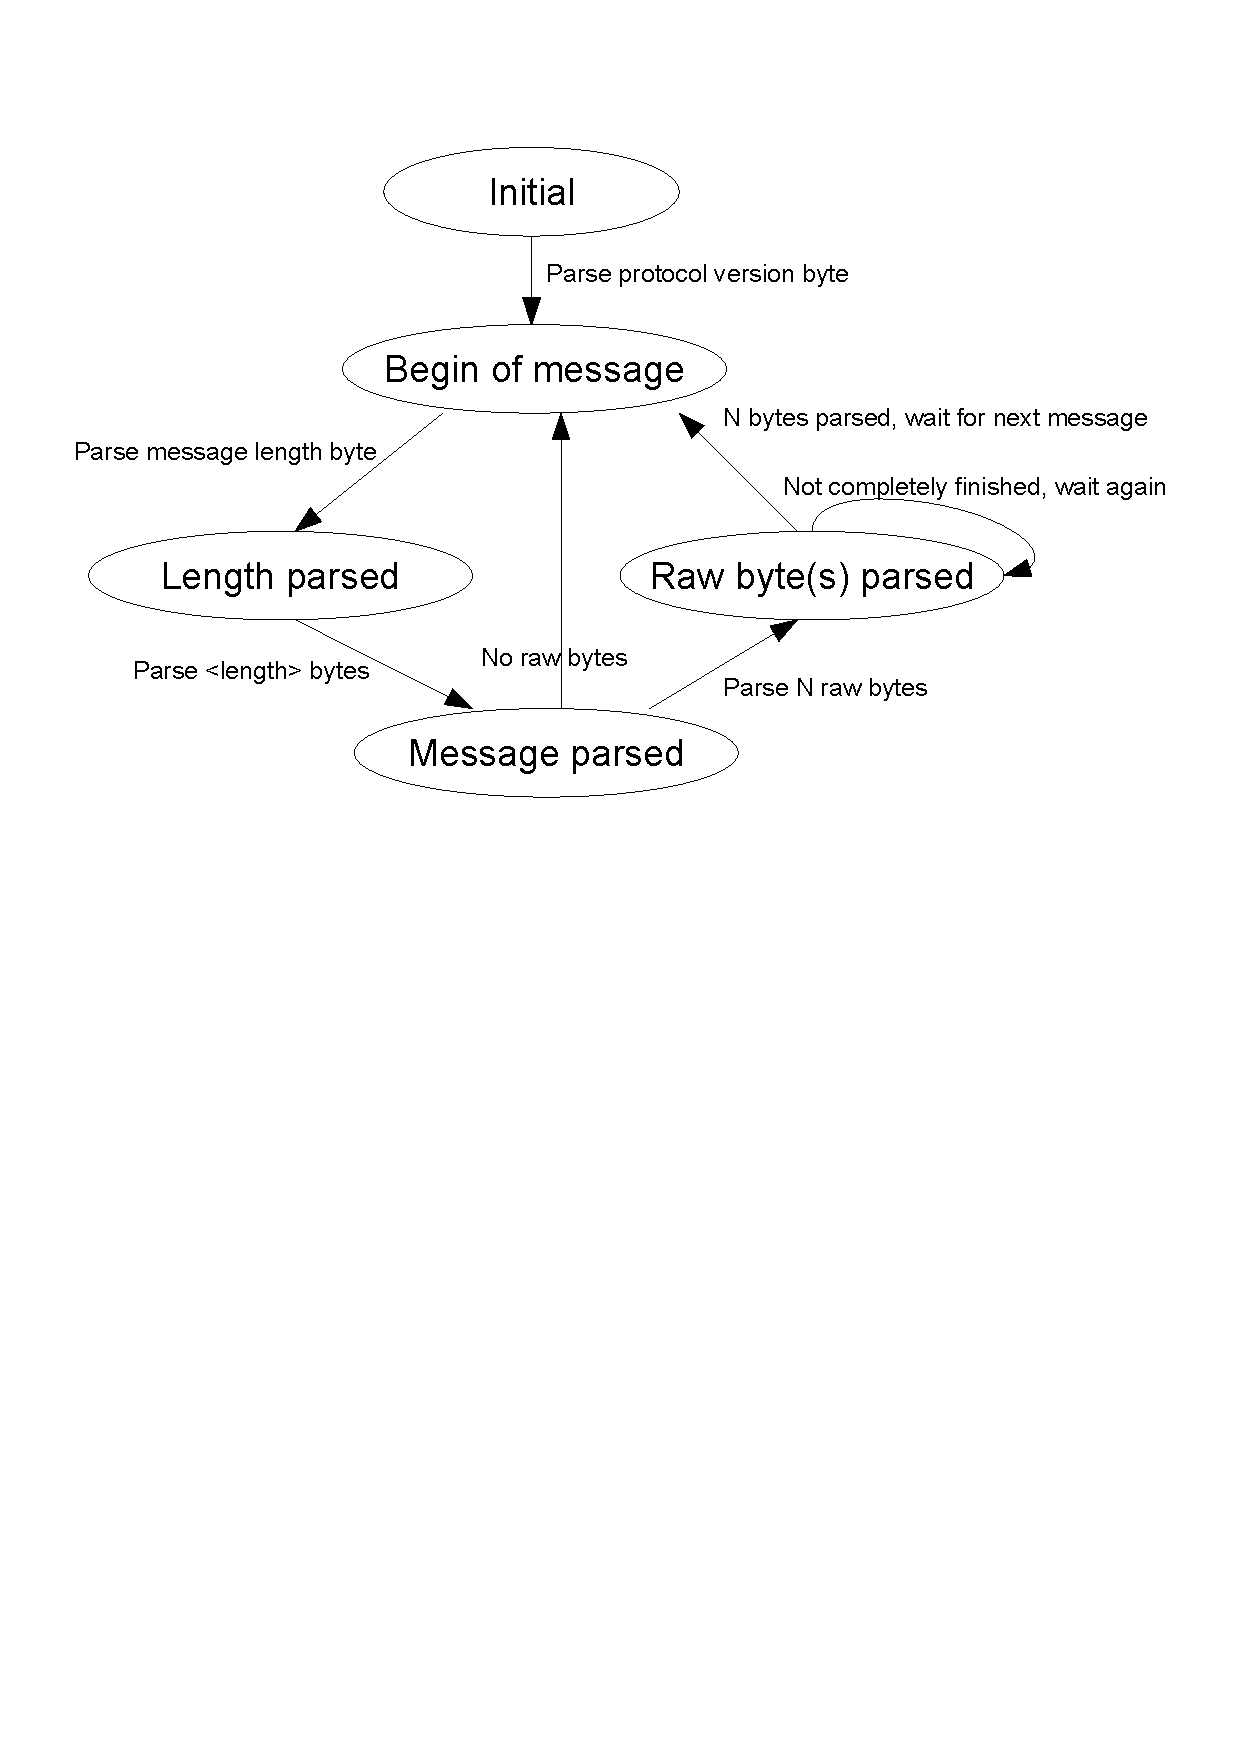
\includegraphics[width=0.9\textwidth,trim=0 16cm 0 1cm,clip=true]{diagrams/parser-statemachine.pdf}
\caption{State machine structure of parser.}
\label{fig:parser-statemachine}
\end{figure}

\paragraph{Replication}
The storage service will store redundant data in order to be failure tolerant as explained in \autoref{sec:state-of-the-art}. A simple but inefficient approach would be to perform exactly the steps as shown in \autoref{fig:xor-replication}. In this way, both storage services must send the data to the parity server (or xor-partner) for a single block that is written by one of the two services. However, the xor-partner is already able to reconstruct the data of the other server that has not performed a write. It only needs to have the old data of the server that has (over)written data. So, in this case mutual exclusion between the two storage services is not an issue anymore, only two times the message size (old data + new data) must be send to the parity server.

Moreover, if we write down this calculation more formal we can conclude that we only have to send the size of the actual message. P stores A1 XOR A2:
\begin{equation}\label{eq1}
\text{P} = \text{A1} \text{ XOR } \text{A2}
\end{equation}
So, lets say we want to store a new value on A1 that is denoted by A1’. The new value of P that is denoted by P’ must be as following:
\begin{equation}\label{eq2}
\text{P’} = \text{A1’} \text{ XOR } \text{A2}
\end{equation}
However, we want to prevent that A2 is necessary for the computation. We can still use the old P and A1, and use (\ref{eq1}) to derive A2 and substitute this in (\ref{eq2}):
$$\text{P’} = \text{A1’} \text{ XOR } \text{A1} \text{ XOR } \text{P}$$
Now, the intermediate result I can be calculated on the server that initiates the XOR-update:
$$\text{I} = \text{A1’} \text{ XOR } \text{A1}$$
Finally, the redundant data server can compute P’:
$$\text{P’} = \text{I} \text{ XOR } \text{P}$$

Release that the above equation assumes that all servers initially start in correct XOR-state. We have decided to use the numerical value zero for all instances in the current implementation ($0$ \verb|xor| $0 = 0$) in combination with a sparse file system to prevent long startup times.

Since a storage service connection allows to stream messages over one single connection. A public storage instance only has to maintain this connection and forward all writes that are xored with the current data to the xor-partner instance.

\paragraph{Management}
The storage instances itself does not guarantee fault-tolerant automatically. If a single storage instance crashes, there must be a system that automatically starts a restore of the lost data. Also, this system must be able to create RAID groups itself, and communicate the correct parity server to each storage instance.

For these management tasks the \verb|StorageManager| component is created. This component is currently not implemented in a redundant way, but this is not a difficult tasks since only two lists (\verb|STAND_BY_LIST| and \verb|ACTIVE_LIST|) must be kept synchronized. Also, it is not a big problem if the storage instance is down for a few seconds, this only means that if in the same time a storage instance also crashes it will not be detected, and thus not restored.

\subsection{Dictionary Service}
\subsection{Freelist Service}
\subsection{Front-end / proxy}
\subsection{Client}
Without the optional front-end layer this layer must know the mapping from dictionary keys to dictionary server instance.

\section{Results}
% discuss also the properties that are explained in the DS lectures
% how fault-tollerant are we?

\section{Future improvements}
% system heavily relies on system clock (signing security) --> internal clock synchronization between components, is not implemented due the lack of time

% storage service:
% Remove blocking code between storageservice and parity server --> show blocking problem by sequence diagram, same for recovery
% Private key meganism, now every server has its own private key which is a big security issue --> only operation,offset,length/data are signed, NOT HOST/PORT!
% Reading from disk in chunks in order to prevent starvation of meerdere threads
% how errors must be handled: storage engine returns one error --> redo entire process, dictionary service will free unwritten entities


%ref: http://twistedmatrix.com/trac/
%ref: http://code.google.com/p/protobuf/

\bibliographystyle{plain}
\bibliography{ref}
\nocite{*}

\end{document}
